% Skeleton only: preamble, section headings, floats pulling from ../figures/.
% The text is written by the author (see README.md in this folder). No AI-written prose here.
% Build: latexmk -pdf main.tex   (from paper/)

% Use the SIAM class when siamart220329.cls is in this folder, else the standard article class.
\newif\ifsiam
\IfFileExists{siamart220329.cls}{\siamtrue\documentclass{siamart220329}}{\documentclass[11pt]{article}}

\usepackage{amsmath}
\usepackage{booktabs}
\usepackage{graphicx}

% Shrink a table to the text width only when it is wider; never enlarge a small one.
\newcommand{\fitwidth}[1]{\resizebox{\ifdim\width>\linewidth\linewidth\else\width\fi}{!}{#1}}

% TODO(author): title and author
\title{TODO(author): title}
\author{TODO(author): name}
\date{}

\begin{document}
\maketitle

\begin{abstract}
% TODO(author): write the abstract.
\end{abstract}

\section{Introduction}
% TODO(author): write. Floats: none planned.

\section{Research question and literature}
% TODO(author): write. Floats: none planned.

\section{Methodology}
% TODO(author): write. Floats: none planned (metrics are defined here, results are in Results).

\section{Data set (source and cleaning)}
% TODO(author): write. Floats for this section:
%   table_pool_filters, table_register_lag, table_adoption_by_type,
%   adoption_by_yield, adoption_by_neighbour_share
\begin{table}[t]
\centering
\caption{Buildings removed by each pool filter at both cut-offs. TODO caption (author).}\label{tab:pool_filters}
\fitwidth{\begin{tabular}{lrrrrrr}
\toprule
 & \multicolumn{3}{c}{Train (cut-off 2021)} & \multicolumn{3}{c}{Test (cut-off 2023)} \\
\cmidrule(lr){2-4} \cmidrule(lr){5-7}
 & Buildings & Adopters & Rate (\%) & Buildings & Adopters & Rate (\%) \\
\midrule
At risk (no PV at the cut-off) & 67{,}482 & 6{,}062 & 9.0 & 61{,}420 & 5{,}234 & 8.5 \\
\midrule
New build & 4{,}049 & 877 & 21.7 & 3{,}172 & 885 & 27.9 \\
No roof record & 5{,}567 & 281 & 5.0 & 5{,}286 & 283 & 5.4 \\
Suitable roof under 20 m$^2$ & 1{,}294 & 57 & 4.4 & 1{,}237 & 46 & 3.7 \\
Pool & 56{,}572 & 4{,}847 & 8.6 & 51{,}725 & 4{,}020 & 7.8 \\
\bottomrule
\end{tabular}
}
\end{table}

\begin{table}[t]
\centering
\caption{First installations by start year in the September and November 2026 plant files. TODO caption (author).}\label{tab:register_lag}
\fitwidth{\begin{tabular}{rrrrr}
\toprule
Start year & September file & November file & Difference & Difference (\%) \\
\midrule
2022 & 2{,}339 & 2{,}340 & 1 & 0.0 \\
2023 & 3{,}714 & 3{,}722 & 8 & 0.2 \\
2024 & 3{,}385 & 3{,}395 & 10 & 0.3 \\
2025 & 1{,}793 & 1{,}839 & 46 & 2.5 \\
\bottomrule
\end{tabular}
}
\end{table}

\begin{table}[t]
\centering
\caption{Buildings and adoption rate by building category and number of dwellings. TODO caption (author).}\label{tab:adoption_by_type}
\fitwidth{\begin{tabular}{p{3.6cm}rrrr}
\toprule
 & \multicolumn{2}{c}{Train (cut-off 2021)} & \multicolumn{2}{c}{Test (cut-off 2023)} \\
\cmidrule(lr){2-3} \cmidrule(lr){4-5}
 & Buildings & Rate (\%) & Buildings & Rate (\%) \\
\midrule
All pool buildings & 56{,}572 & 8.6 & 51{,}725 & 7.8 \\
\midrule
\multicolumn{5}{l}{\textit{Building category (gkat)}} \\
Residential only (1020) & 47{,}161 & 9.4 & 42{,}734 & 8.5 \\
Residential with ancillary use (1030) & 6{,}863 & 4.7 & 6{,}540 & 4.6 \\
Partly residential (1040) & 2{,}548 & 3.8 & 2{,}451 & 4.2 \\
\multicolumn{5}{l}{\textit{Number of dwellings}} \\
1 & 37{,}438 & 9.9 & 33{,}742 & 8.6 \\
2 & 9{,}657 & 8.1 & 8{,}877 & 8.0 \\
3 & 3{,}021 & 6.2 & 2{,}835 & 5.9 \\
4 or more & 6{,}272 & 2.9 & 6{,}091 & 3.9 \\
Not recorded & 184 & 2.2 & 180 & 3.9 \\
\bottomrule
\end{tabular}
}
\end{table}

\begin{figure}[t]
\centering
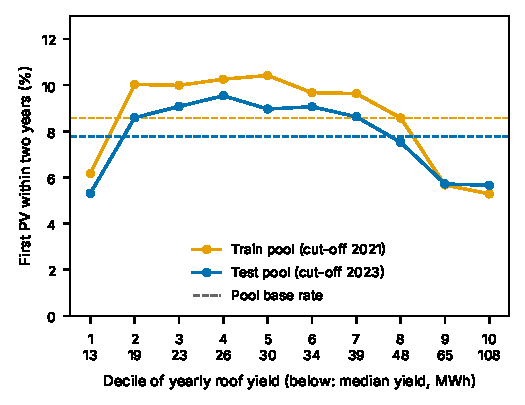
\includegraphics[width=\linewidth]{../figures/adoption_by_yield.pdf}
\caption{Adoption rate by decile of yearly roof yield. TODO caption (author).}\label{fig:adoption_by_yield}
\end{figure}

\begin{figure}[t]
\centering
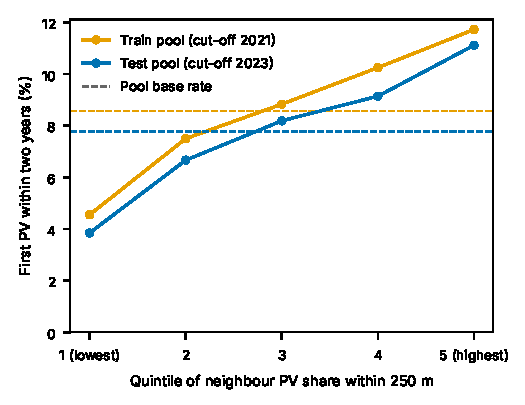
\includegraphics[width=\linewidth]{../figures/adoption_by_neighbour_share.pdf}
\caption{Adoption rate by quintile of the neighbour PV share at 250 m. TODO caption (author).}\label{fig:adoption_by_neighbour_share}
\end{figure}

\section{Implementation}
% TODO(author): write. Floats: none planned.

\section{Results}
% TODO(author): write. Floats for this section:
%   table_metrics, table_metrics_rank, capture_curve, table_model_gaps,
%   table_lasso_coef, lasso_cv, map_adoption, gp_residual_map,
%   table_segments, pca_segments, table_heating_leak
\begin{table}[t]
\centering
\caption{Capture at 5\% and 10\% on the test pool. TODO caption (author).}\label{tab:metrics}
\fitwidth{\begin{tabular}{p{3.4cm}rr}
\toprule
Model & Capture at 5\% & Capture at 10\% \\
\midrule
Random & 0.050 & 0.100 \\
Roof yield & 0.036 [0.030, 0.043] & 0.073 [0.064, 0.080] \\
Neighbour PV share & 0.066 [0.057, 0.074] & 0.131 [0.119, 0.146] \\
LASSO & 0.099 [0.090, 0.109] & 0.195 [0.179, 0.214] \\
Neural net (16) & 0.098 [0.087, 0.108] & 0.194 [0.175, 0.210] \\
Neural net (32, 16) & 0.100 [0.089, 0.111] & 0.192 [0.177, 0.207] \\
\midrule
\multicolumn{3}{l}{\textit{Sensitivity runs with heating (leakage, upper bound)}} \\
LASSO + heating source & 0.142 [0.129, 0.155] & 0.245 [0.229, 0.259] \\
LASSO + heating source and date & 0.140 [0.130, 0.150] & 0.253 [0.241, 0.269] \\
\bottomrule
\end{tabular}
}
\end{table}

\begin{table}[t]
\centering
\caption{ROC AUC and average precision on the test pool. TODO caption (author).}\label{tab:metrics_rank}
\fitwidth{\begin{tabular}{p{3.4cm}rr}
\toprule
Model & ROC AUC & Average precision \\
\midrule
Random & 0.500 & 0.078 \\
Roof yield & 0.481 [0.469, 0.493] & 0.072 [0.067, 0.076] \\
Neighbour PV share & 0.598 [0.580, 0.616] & 0.099 [0.094, 0.104] \\
LASSO & 0.664 [0.648, 0.678] & 0.129 [0.122, 0.139] \\
Neural net (16) & 0.661 [0.642, 0.674] & 0.126 [0.119, 0.135] \\
Neural net (32, 16) & 0.661 [0.646, 0.674] & 0.129 [0.122, 0.137] \\
\midrule
\multicolumn{3}{l}{\textit{Sensitivity runs with heating (leakage, upper bound)}} \\
LASSO + heating source & 0.720 [0.706, 0.731] & 0.166 [0.157, 0.176] \\
LASSO + heating source and date & 0.720 [0.706, 0.732] & 0.169 [0.159, 0.181] \\
\bottomrule
\end{tabular}
}
\end{table}

\begin{figure}[t]
\centering
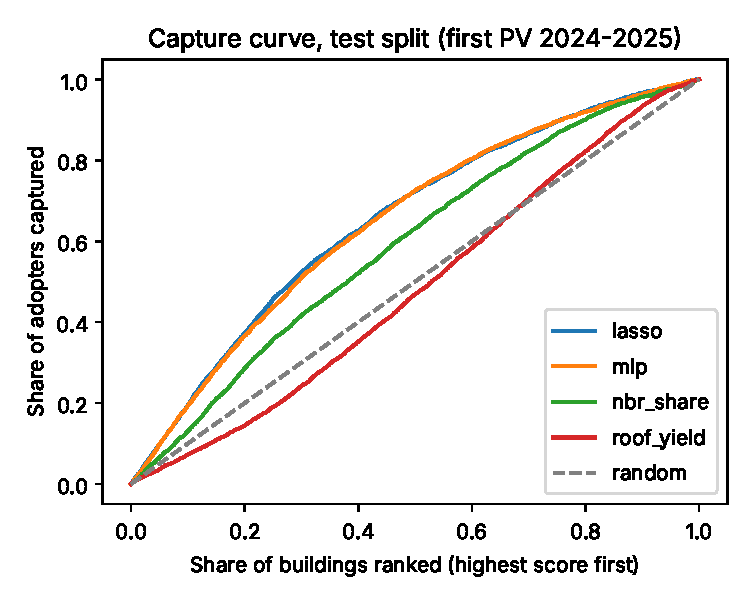
\includegraphics[width=\linewidth]{../figures/capture_curve.pdf}
\caption{Capture curve on the test pool. TODO caption (author).}\label{fig:capture_curve}
\end{figure}

% Wide rows: scaled to the text width. Check legibility once the text is written.
\begin{table}[t]
\centering
\footnotesize
\caption{Paired gaps between models. TODO caption (author).}\label{tab:model_gaps}
\fitwidth{\begin{tabular}{llrr}
\toprule
Label & Gap (first minus second) & Capture at 10\% & ROC AUC \\
\midrule
Test, first PV 2024-2025 & lasso minus nbr share & 0.064 [0.048, 0.079] & 0.066 [0.054, 0.079] \\
Test, first PV 2024-2025 & lasso minus roof yield & 0.122 [0.102, 0.141] & 0.183 [0.159, 0.205] \\
Test, first PV 2024-2025 & nbr share minus roof yield & 0.058 [0.044, 0.077] & 0.117 [0.095, 0.138] \\
\midrule
Test, first PV 2024 only & lasso minus nbr share & 0.077 [0.060, 0.093] & 0.068 [0.058, 0.080] \\
Test, first PV 2024 only & lasso minus roof yield & 0.142 [0.121, 0.170] & 0.195 [0.171, 0.219] \\
Test, first PV 2024 only & nbr share minus roof yield & 0.066 [0.048, 0.089] & 0.127 [0.104, 0.151] \\
\bottomrule
\end{tabular}
}
\end{table}

\begin{table}[t]
\centering
\caption{The 25 largest non-zero LASSO coefficients. TODO caption (author).}\label{tab:lasso_coef}
\fitwidth{\begin{tabular}{lr}
\toprule
Feature (standardised) & Coefficient \\
\midrule
Three or more dwellings (gklas 1122) & -0.388 \\
Log footprint & 0.323 \\
Built before 1919 (gbaup 8011) & -0.260 \\
Partly residential (gkat 1040) & -0.242 \\
Built 1919 to 1945 (gbaup 8012) & -0.171 \\
Dwelling count: 3 & 0.161 \\
Residential only (gkat 1020) & 0.152 \\
Dwelling count: 4 or more & -0.139 \\
Built 2011 to 2015 (gbaup 8022) & 0.130 \\
Built 1961 to 1970 (gbaup 8014) & -0.120 \\
Log suitable roof area, squared & -0.117 \\
Built 1946 to 1960 (gbaup 8013) & -0.116 \\
Neighbour PV share, 250 m & 0.101 \\
Built 2006 to 2010 (gbaup 8021) & 0.100 \\
Building class not recorded & 0.092 \\
Two dwellings (gklas 1121) & -0.092 \\
Built 1996 to 2000 (gbaup 8019) & 0.089 \\
Built 1971 to 1980 (gbaup 8015) & -0.083 \\
Dwelling count: 2 & 0.082 \\
Built 2001 to 2005 (gbaup 8020) & 0.082 \\
Best roof class 5 & 0.073 \\
Suitable share of roof area & 0.065 \\
Roof yield, train decile 1 & -0.063 \\
Neighbour PV share, 100 m & 0.062 \\
Built after 2015 (gbaup 8023) & 0.054 \\
\midrule
\multicolumn{2}{l}{$C = 0.1000$, 44 of 51 coefficients non-zero, mean CV AUC 0.6777} \\
\bottomrule
\end{tabular}
}
\end{table}

\begin{figure}[t]
\centering
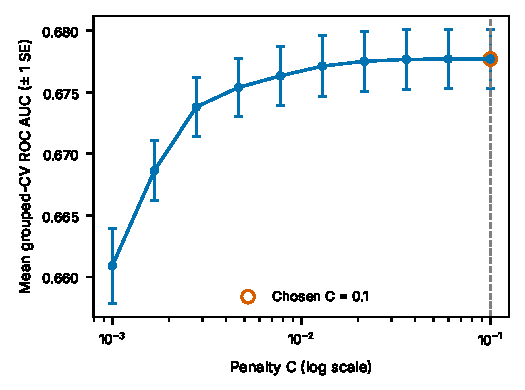
\includegraphics[width=\linewidth]{../figures/lasso_cv.pdf}
\caption{Grouped cross-validation curve of the LASSO. TODO caption (author).}\label{fig:lasso_cv}
\end{figure}

\begin{figure}[t]
\centering
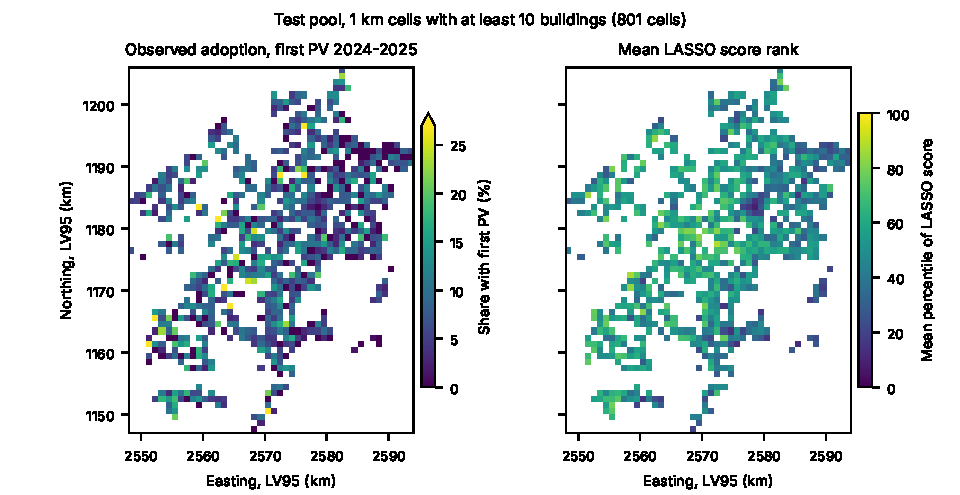
\includegraphics[width=\linewidth]{../figures/map_adoption.pdf}
\caption{Observed adoption rate and mean LASSO score percentile per 1 km cell, test pool. TODO caption (author).}\label{fig:map_adoption}
\end{figure}

\begin{figure}[t]
\centering
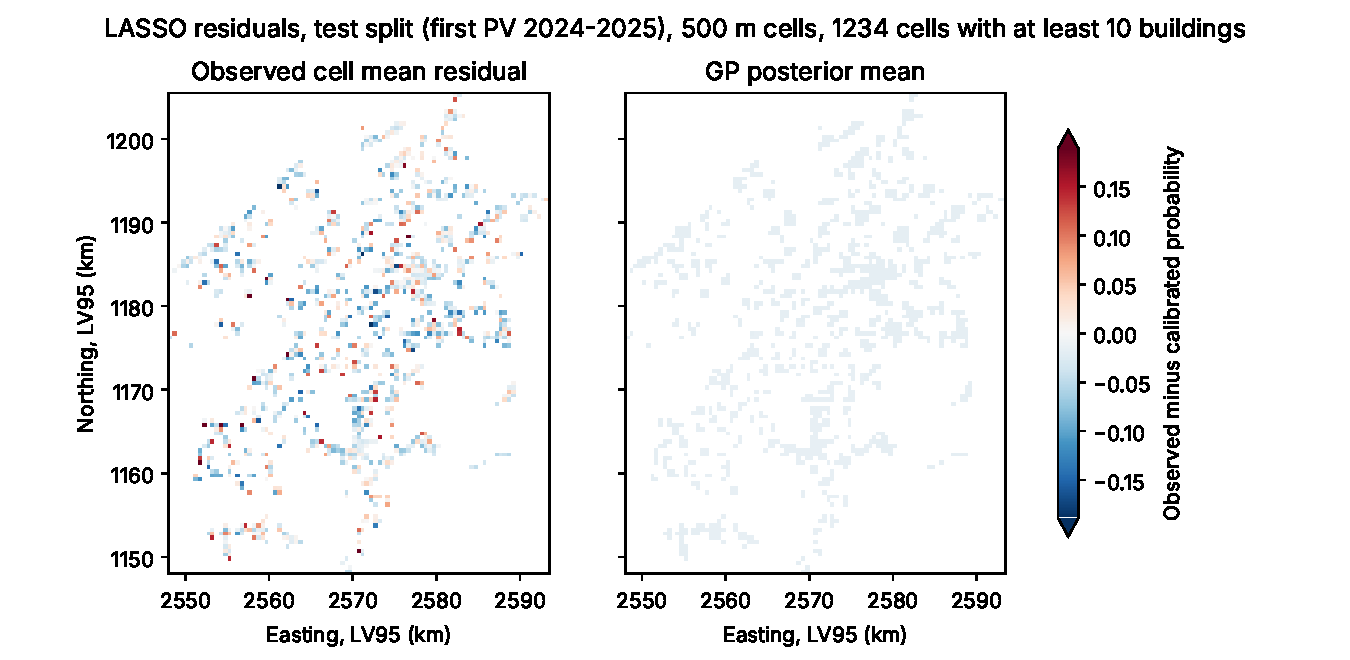
\includegraphics[width=\linewidth]{../figures/gp_residual_map.pdf}
\caption{Observed and GP-smoothed LASSO residual per 500 m cell, test pool. TODO caption (author).}\label{fig:gp_residual_map}
\end{figure}

% 11 columns: scaled to the text width.
\begin{table}[t]
\centering
\footnotesize
\caption{K-means segments. TODO caption (author).}\label{tab:segments}
\fitwidth{\begin{tabular}{llrrrrrrrrr}
\toprule
 & & \multicolumn{2}{c}{Train (cut-off 2021)} & \multicolumn{2}{c}{Test (cut-off 2023)} & \multicolumn{5}{c}{Mean on train} \\
\cmidrule(lr){3-4} \cmidrule(lr){5-6} \cmidrule(lr){7-11}
Segment & Description & Buildings & Adoption (\%) & Buildings & Adoption (\%) & Dwellings & Floors & Suitable roof (m$^2$) & Yield (MWh/yr) & Suitable share of roof \\
\midrule
1 &  & 21{,}505 & 9.0 & 19{,}369 & 7.8 & 1.3 & 2.3 & 102 & 23 & 0.53 \\
2 &  & 19{,}823 & 11.1 & 18{,}153 & 10.0 & 1.2 & 2.1 & 175 & 35 & 0.95 \\
3 &  & 9{,}413 & 5.9 & 8{,}612 & 5.8 & 1.7 & 2.3 & 433 & 91 & 0.69 \\
4 &  & 5{,}831 & 2.7 & 5{,}591 & 3.6 & 5.6 & 4.0 & 384 & 79 & 0.82 \\
\bottomrule
\end{tabular}
}
\end{table}

\begin{figure}[t]
\centering
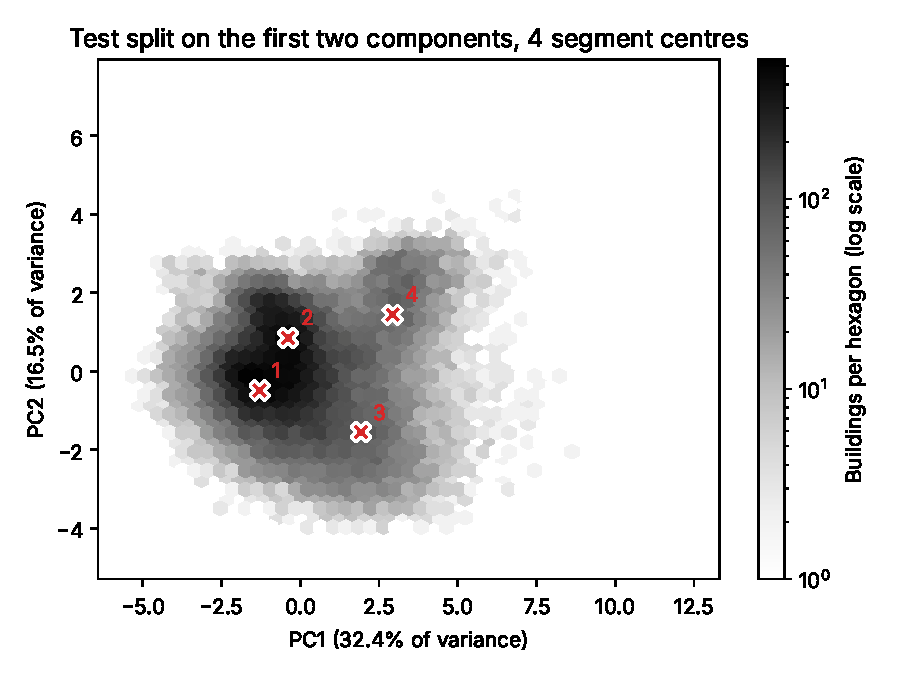
\includegraphics[width=\linewidth]{../figures/pca_segments.pdf}
\caption{Test pool on the first two principal components with the segment centres. TODO caption (author).}\label{fig:pca_segments}
\end{figure}

\begin{table}[t]
\centering
\caption{Adoption by date of the heating record. TODO caption (author).}\label{tab:heating_leak}
\fitwidth{\begin{tabular}{lrrrrrr}
\toprule
 & \multicolumn{3}{c}{Train (cut-off 2021)} & \multicolumn{3}{c}{Test (cut-off 2023)} \\
\cmidrule(lr){2-4} \cmidrule(lr){5-7}
 & Buildings & Adopters & Rate (\%) & Buildings & Adopters & Rate (\%) \\
\midrule
Heating record dated after the cut-off & 15{,}523 & 2{,}368 & 15.3 & 6{,}202 & 810 & 13.1 \\
Heating record dated up to the cut-off & 40{,}936 & 2{,}477 & 6.1 & 45{,}412 & 3{,}206 & 7.1 \\
No heating date & 113 & 2 & 1.8 & 111 & 4 & 3.6 \\
\midrule
Pool & 56{,}572 & 4{,}847 & 8.6 & 51{,}725 & 4{,}020 & 7.8 \\
\bottomrule
\end{tabular}
}
\end{table}

\section{Conclusion}
% TODO(author): write. Floats: none planned.

% TODO(author): references (bibliography) go here, after the conclusion and before the appendix.

\appendix
\section{Declaration of tools}
% TODO(author): write the declaration from docs/ai_log.md (what was asked of AI sessions, files
% touched) and docs/decisions.md (choices). Also list code from outside sources (CLAUDE.md, Course rules).
% Floats for this section (supplementary tables):
%   table_metrics_2024, table_metrics_2024_rank, table_lasso_coef_full
\begin{table}[t]
\centering
\caption{Capture at 5\% and 10\%, first PV in 2024 only. TODO caption (author).}\label{tab:metrics_2024}
\fitwidth{\begin{tabular}{p{3.4cm}rr}
\toprule
Model & Capture at 5\% & Capture at 10\% \\
\midrule
Random & 0.050 & 0.100 \\
Roof yield & 0.034 [0.027, 0.042] & 0.067 [0.058, 0.076] \\
Neighbour PV share & 0.066 [0.056, 0.076] & 0.133 [0.119, 0.151] \\
LASSO & 0.104 [0.092, 0.114] & 0.210 [0.190, 0.235] \\
Neural net (16) & 0.101 [0.089, 0.114] & 0.200 [0.178, 0.219] \\
Neural net (32, 16) & 0.103 [0.091, 0.117] & 0.204 [0.185, 0.223] \\
\midrule
\multicolumn{3}{l}{\textit{Sensitivity runs with heating (leakage, upper bound)}} \\
LASSO + heating source & 0.138 [0.123, 0.151] & 0.244 [0.229, 0.259] \\
LASSO + heating source and date & 0.135 [0.123, 0.149] & 0.255 [0.237, 0.276] \\
\bottomrule
\end{tabular}
}
\end{table}

\begin{table}[t]
\centering
\caption{ROC AUC and average precision, first PV in 2024 only. TODO caption (author).}\label{tab:metrics_2024_rank}
\fitwidth{\begin{tabular}{p{3.4cm}rr}
\toprule
Model & ROC AUC & Average precision \\
\midrule
Random & 0.500 & 0.052 \\
Roof yield & 0.480 [0.468, 0.494] & 0.047 [0.044, 0.051] \\
Neighbour PV share & 0.607 [0.588, 0.626] & 0.068 [0.064, 0.072] \\
LASSO & 0.675 [0.656, 0.690] & 0.091 [0.084, 0.098] \\
Neural net (16) & 0.666 [0.647, 0.681] & 0.086 [0.080, 0.093] \\
Neural net (32, 16) & 0.669 [0.650, 0.684] & 0.089 [0.084, 0.096] \\
\midrule
\multicolumn{3}{l}{\textit{Sensitivity runs with heating (leakage, upper bound)}} \\
LASSO + heating source & 0.720 [0.704, 0.735] & 0.111 [0.104, 0.119] \\
LASSO + heating source and date & 0.720 [0.703, 0.733] & 0.112 [0.104, 0.121] \\
\bottomrule
\end{tabular}
}
\end{table}

% 44 rows: [p] puts it on its own page; footnotesize keeps it on one page.
\begin{table}[p]
\centering
\footnotesize
\caption{All non-zero LASSO coefficients. TODO caption (author).}\label{tab:lasso_coef_full}
\fitwidth{\begin{tabular}{lr}
\toprule
Feature (standardised) & Coefficient \\
\midrule
Three or more dwellings (gklas 1122) & -0.388 \\
Log footprint & 0.323 \\
Built before 1919 (gbaup 8011) & -0.260 \\
Partly residential (gkat 1040) & -0.242 \\
Built 1919 to 1945 (gbaup 8012) & -0.171 \\
Dwelling count: 3 & 0.161 \\
Residential only (gkat 1020) & 0.152 \\
Dwelling count: 4 or more & -0.139 \\
Built 2011 to 2015 (gbaup 8022) & 0.130 \\
Built 1961 to 1970 (gbaup 8014) & -0.120 \\
Log suitable roof area, squared & -0.117 \\
Built 1946 to 1960 (gbaup 8013) & -0.116 \\
Neighbour PV share, 250 m & 0.101 \\
Built 2006 to 2010 (gbaup 8021) & 0.100 \\
Building class not recorded & 0.092 \\
Two dwellings (gklas 1121) & -0.092 \\
Built 1996 to 2000 (gbaup 8019) & 0.089 \\
Built 1971 to 1980 (gbaup 8015) & -0.083 \\
Dwelling count: 2 & 0.082 \\
Built 2001 to 2005 (gbaup 8020) & 0.082 \\
Best roof class 5 & 0.073 \\
Suitable share of roof area & 0.065 \\
Roof yield, train decile 1 & -0.063 \\
Neighbour PV share, 100 m & 0.062 \\
Built after 2015 (gbaup 8023) & 0.054 \\
Other building class & 0.045 \\
Floors & 0.044 \\
Best roof class 3 & -0.041 \\
Built 1986 to 1990 (gbaup 8017) & 0.040 \\
Built 1991 to 1995 (gbaup 8018) & 0.037 \\
Dwelling count not recorded & -0.036 \\
Log (1 + buildings within 250 m) & 0.029 \\
Roof yield, train decile 5 & 0.024 \\
Roof yield, train decile 9 & -0.022 \\
Construction period not recorded & 0.018 \\
Roof yield, train decile 10 & -0.017 \\
Footprint not recorded & -0.016 \\
Roof yield, train decile 7 & 0.015 \\
Floors not recorded & -0.012 \\
Tariff minus canton median & 0.012 \\
Roof yield, train decile 2 & 0.011 \\
Roof yield, train decile 8 & 0.009 \\
Roof yield, train decile 4 & 0.008 \\
Roof yield, train decile 6 & -0.005 \\
\midrule
\multicolumn{2}{l}{$C = 0.1000$, 44 of 51 coefficients non-zero, mean CV AUC 0.6777} \\
\bottomrule
\end{tabular}
}
\end{table}

\end{document}
